\section{Introduction}

Action recognition in videos is crucial in computer vision as it enables the analysis and interpretation of human activity. These actions are inherently sequential, consisting of interconnected events. Typically, tasks in video understanding include video classification \cite{2014_vc_karpathy, 2014_vc_simonyan, 2017_quovadis, 2020_x3d, 2021_vivit, 2021_videoclass_actionclip}, which involves mapping a global video representation to an action category, or action detection \cite{2017_actiondetect, 2018_videocapsulenet, 2019_slowfast, 2018_bsn, 2022_actionformer}, which aims to identify both the spatial and temporal boundaries of specific actions within a video.
However, these methods present several challenges: (i) Most approaches require fine-grained annotations, which are time-consuming and labor-intensive; (ii) Most approaches struggle to capture the complex temporal information and causal relationships that vary across diverse videos.
To address these challenges, we explore how representation learning based on the pretext-task of video alignment can improve performance in downstream action recognition tasks such as action phase classification and action progression.

Prior self-supervised or weakly-supervised video alignment approaches \cite{2017_tcn, 2019_tcc, 2021_lav, 2021_gta, 2022_carl, 2024_lrprop} train on pairs of videos that describe the same action using either cycle-consistency \cite{2019_tcc}, soft dynamic time warping \cite{2021_gta, 2021_lav}, or sequential contrastive learning \cite{2022_carl}.
We notice that the pretext task of video alignment shares similarities with bioinformatics sequence alignment for studying DNA, RNA, and protein structures. 
Since some actions are composed of sub-actions or events that occur in a specific order, video alignment shares similarities with protein alignment, as both involve identifying regions of continuity and discontinuity within sequences.
There are two main types of alignment algorithms commonly used in bioinformatics: \textit{global} and \textit{local}. 
The Needleman-Wunsch (NW) algorithm \cite{1970_nw}, a global alignment method, aligns entire sequences from start to finish. 
This approach is conceptually similar to Dynamic Time Warping (DTW) \cite{2007_dtw}, which aligns sequences of varying lengths by matching their temporal patterns from start to finish.
Differentiable versions of NW and DTW algorithms have been established by incorporating smooth maximum/minimum and argmax/argmin functions \cite{2020_diff_nw, 2017_softdtw}.
In particular, Soft-DTW \cite{2017_softdtw} has been used in prior video alignment approaches \cite{2021_lav, 2021_gta, 2024_lrprop}.
In contrast, the Smith-Waterman (SW) algorithm \cite{1981_sw}, which implements local alignment, identifies regions of high similarity within sequences and is adaptable to gaps, insertions, and deletions. 
This capability to handle subsequences makes local alignment particularly appropriate for managing the complexities of action recognition in realistic settings. 
Recently, bioinformatics research has introduced a differentiable form of the SW algorithm \cite{2023_sw1, 2023_sw2}, which we adopt for the first time in the context of representation learning to align video sequences.

Specifically, in this work, we introduce a novel loss function termed \textit{Local-Alignment Contrastive} (LAC) loss, integrated into our proposed end-to-end framework for the video alignment task, as visualized in Fig. \ref{fig: vis_intro}.
Following prior works \cite{2022_carl, 2024_lrprop}, our framework uses a variation of convolutional and transformer encoders to extract spatio-temporal features from each frame. 
Our novel LAC loss enables the comparison of video pairs through a consistent and differentiable local alignment loss. 
This loss specifically accommodates sequences with learned penalties for opening gaps and extending them, combined with a contrastive loss that effectively separates dissimilar frames.
We demonstrate that the learned representations of our approach outperform previous methods on various downstream action recognition tasks, such as action phase classification and action phase progression on the Pouring~\cite{2017_tcn} and PennAction~\cite{2013_pennaction} datasets. 

\begin{figure}[t]
\begin{tabular}{c}
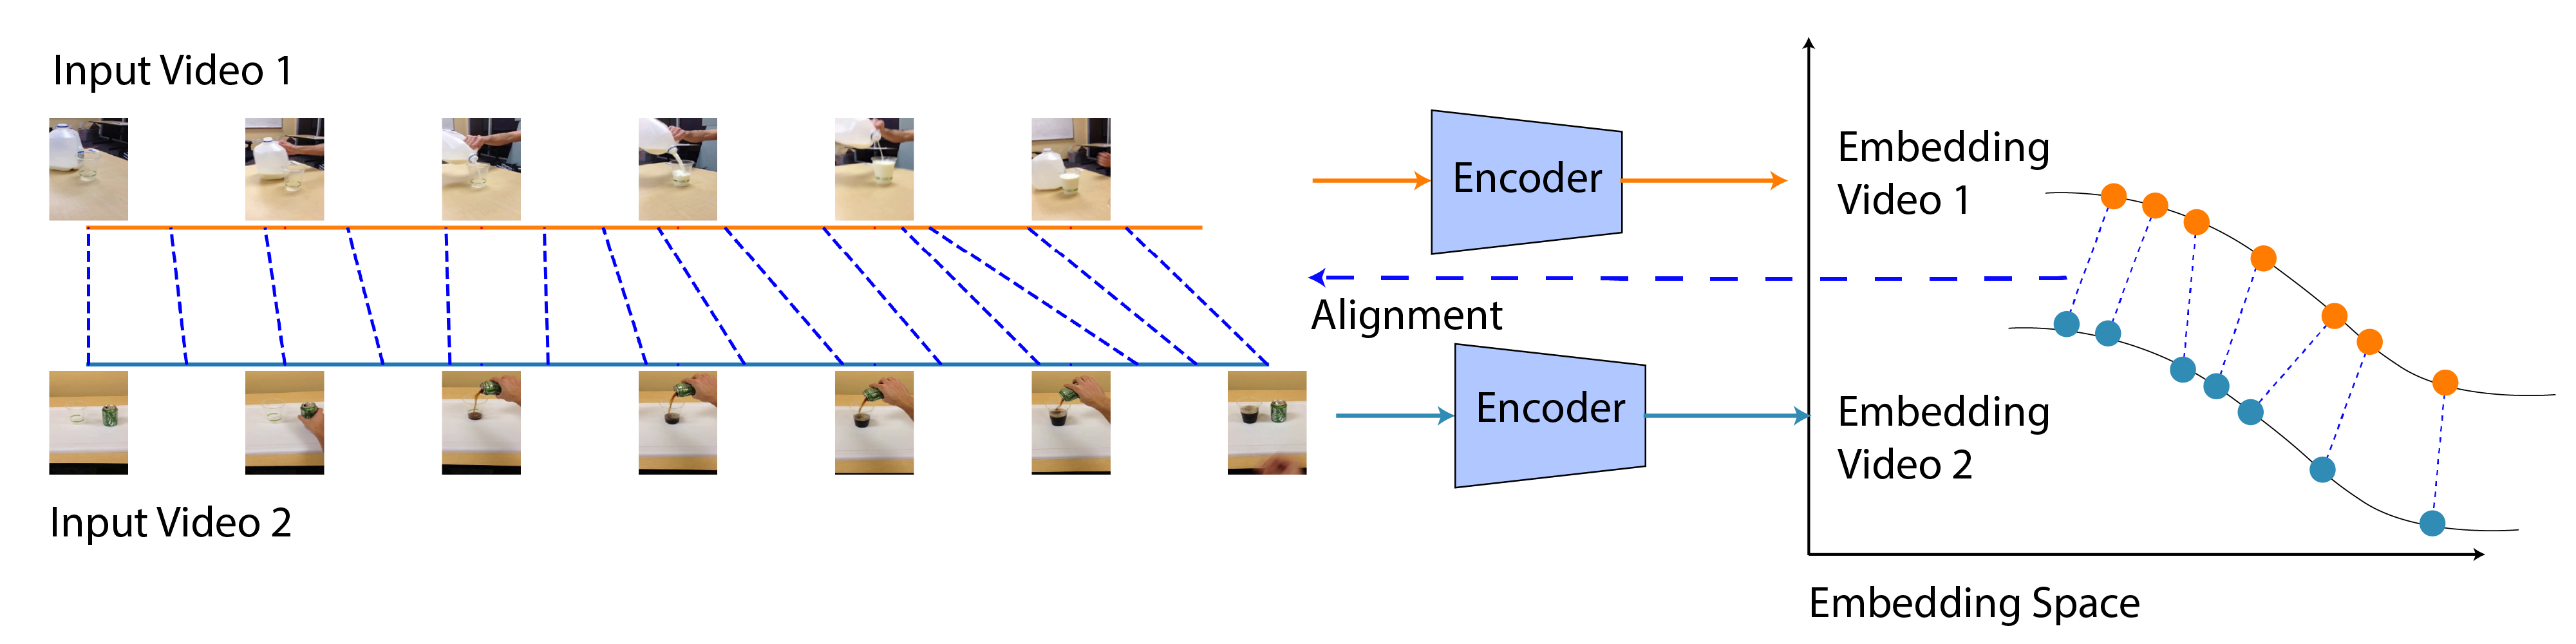
\includegraphics[width=\textwidth]{images/a1.png}
\end{tabular}
\caption{We introduce a representation learning approach that aligns video sequences depicting the same processes. Our training objective is to use a novel LAC loss to optimize and learn an element-wise embedding function that supports the alignment process.}
\label{fig: vis_intro}
\end{figure}
